\documentclass{article}
\usepackage{hyperref}
\usepackage[linguistics]{forest}
\usepackage{graphicx}
\usepackage[margin=1in]{geometry}
\usepackage{adjustbox}
\usepackage{bookmark}
\usepackage{rotating}
\usepackage{amsmath}

\title{Homework \#1\\ 
    \vspace{0.5cm}
    \normalsize John Karasev\\
    \vspace{0.2cm}
    \normalsize STAT 672\\
    \vspace{0.2cm}
    January 22, 2020 }
\date{}
\begin{document}
\maketitle

\section{Orthogonal projection in a hilbert space}
\[\pi_V(f) \in V;\]
\[\langle f - \pi_V(f), g \rangle =0 \ \forall g \in V; \]
\begin{enumerate}
    \item   
        \begin{equation}
        \begin{aligned}
        \|f\|^2 &= \langle f, f \rangle \\
        & = \langle \pi_v(f) + (f - \pi_v(f)), \pi_v(f) + (f - \pi_v(f)) \rangle  \notag \\
        & = \langle \pi_v(f), \pi_v(f) \rangle + 2\langle \pi_v(f), f - \pi_v(f) \rangle + \langle f - \pi_v(f), f - \pi_v(f) \rangle \notag \\
        & = \|\pi_v(f)\|^2 + \|f - \pi_v(f)\|^2\ center\ term\ cancels\ since\ orthogonal 
        \end{aligned}
        \end{equation}
    \item 
        \begin{equation}
        \begin{aligned}
        \langle f, \pi_v(g) \rangle &= \langle (f-\pi_v(f)) + \pi_v(f), \pi_v(g) \rangle \\
        & = \langle f-\pi_v(f) , \pi_v(g) \rangle +  \langle \pi_v(f) , \pi_v(g) \rangle \notag \\
        & = \langle \pi_v(f) , \pi_v(g) \rangle\ by\ orthogonality
        \end{aligned}
        \end{equation} 
        
        \begin{equation}
        \begin{aligned}
        \langle g, \pi_v(f) \rangle &= \langle (g-\pi_v(g)) + \pi_v(g), \pi_v(f) \rangle \\
        & = \langle g-\pi_v(g), \pi_v(f) \rangle +  \langle \pi_v(g) , \pi_v(f) \rangle \notag \\
        & = \langle \pi_v(g) , \pi_v(f) \rangle\ by\ orthogonality
        \end{aligned}
        \end{equation}

        \[ \langle g, \pi_v(f) \rangle = \langle f, \pi_v(g) \rangle\]
    \item 
\end{enumerate}


\section{A reproducing kernel is positive definite}
\begin{enumerate}
    \item 
        \[K(x,y) = \langle K_x(y), K_y(x) \rangle\ by\ reproducing\ property\]
        \[K(y,x) = \langle K_y(y), K_x(x) \rangle\ by\ reproducing\ property\] 
        \[K(x,y) = K(y,x)\]
    \item
        \begin{equation}
        \begin{aligned}
        K(x,y) & = \langle K_x(y), K_y(x) \rangle\\
        & =  \langle K_y(x), K_y(x) \rangle \ge 0\ by\ symmetry\notag \\
        \end{aligned}
        \end{equation}
    \item 
        \begin{equation}
        \begin{aligned}
        |f(x)| & \le \|f\|\sqrt{K(x,x)}\\
        |\langle f, K_x \rangle|& \le  \|f\| \sqrt{\langle K_x, K_x \rangle} \notag \\
        |\langle f, K_x \rangle|& \le  \|f\| \| K_x \|\ true\ by\ Cauchy-Schwartz\ inequality \notag \\
        \end{aligned}
        \end{equation}

\end{enumerate}

\section{RKHS over a finite set}
\begin{enumerate}
    \item 
        

\end{enumerate}

\vspace{0.5cm}

\adjustbox{valign=t}{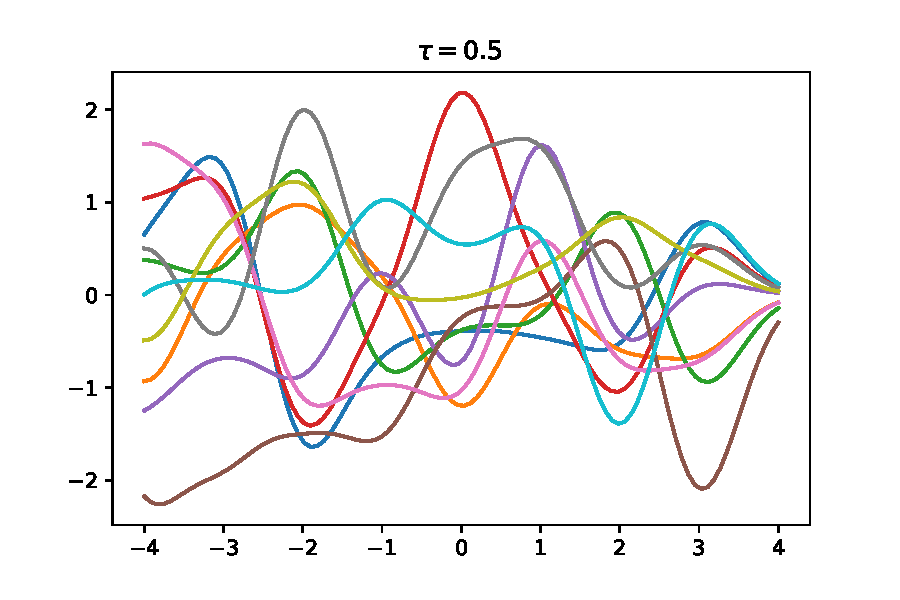
\includegraphics[width=15cm]{../figures/gausst0_5.pdf}}

\vspace{0.5cm}


\end{document}
